\subsection{Consistency of local Voronoi diagrams}
\label{sec:localVoronoi}

In this section, we prove that the local and global Voronoi diagrams are the same within a particular distance from LiDAR.
%
A part of the track boundaries may not be \emph{visible} due to two reasons: being out of LiDAR's range, or occluded by other track boundaries.


Let $R$ be the range of LiDAR, 
and $d$ be the minimum distance of the track boundaries to LiDAR.
%
If $d \leq R$ then at least one point on the track boundaries is visible to LiDAR, so the local Voronoi diagram can be defined.
%
For any visible point $v$ on the track boundaries we have $d \leq \lVert v \rVert \leq R$ where $ \lVert \cdot \rVert $ is the Euclidean norm in LiDAR's coordinates.
%
We have the following guarantees:

\begin{figure}
\centering
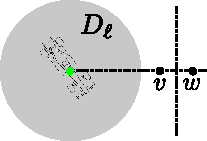
\includegraphics[width=4cm]{Figures/voronoi_occlusion.pdf}
\caption{If the Voronoi cell of a point in $D_\ell$ is identified by a track boundary $w$, then no track boundary $v$ occludes $w$. The green dot is LiDAR.}
\label{fig:voronoi-global-to-local}
\end{figure}

\begin{theorem}
Suppose that $d \leq R$.
%
Then the local and global Voronoi diagrams coincide on the disk $D_\ell$ of radius $\ell$ centered at LiDAR where
$$
\ell = \min \{ \frac{R-d}{2}, d \}.
$$
\label{thm:voronoi}
\end{theorem}

\begin{proof}
Let $p \in D_\ell$.
%
The global Voronoi cell of $p$ is identified with its closest track boundary points.
%
To prove that the local Voronoi cell of $p$ is the same as its global Voronoi cell, it is sufficient to show that all track boundary points closest to $p$ are visible.


Let $w$ be a track boundary closest to $p$.
%
We need to show that $w$ is visible.
%
By definition of $d$, there is a track boundary point $u$ with $\lVert u \rVert = d$.
%
By choice of $w$, we have
$$
\lVert p - w \rVert 
\leq \lVert p - u \rVert 
\leq \lVert p \rVert + \lVert u \rVert \leq \ell + d
$$
%
By definition of $\ell$, we have $\ell \leq \frac{R-d}{2}$, so
$$
\lVert w \rVert = \lVert w - p + p \rVert \leq \lVert w-p \rVert + \lVert p \rVert \leq 2\ell+d \leq R.
$$
%
This proves that $w$ is in range of LiDAR.
%
It remains to show that $w$ is not occluded.

Suppose, for the sake of contradiction, that $w$ is occluded.
%
That is,
there is a track boundary on the line segment between LiDAR and $w$.
%
Clearly, such points are in range since they are closer than $w$.
%
Choose $v$ to be such an occluding point that is the closest to LiDAR, so that $v$ is visible.
%
We must have $d \leq \lVert v \rVert $, by the definition of $d$.
%
Therefore, $\ell \leq d \leq \lVert v \rVert $.
%
Hence, all points in $D_\ell$ are closer to $v$ than to $w$, as shown in Fig~\ref{fig:voronoi-global-to-local}, since $D_\ell$ is on the left of the perpendicular bisector of the segment $vw$. 
%
In particular, $p$ is closer to $v$ than to $w$, which contradicts the choice of $w$.
%
Therefore, no such $v$ exists and $w$ is not occluded.
\end{proof}

Note that $D_\ell$ may not necessarily contain Voronoi \emph{edges} i.e. points that are equidistant from two or more different track boundary points.
%
Our planner chooses a path on the Voronoi edges so we need to make sure that $D_\ell$ contains Voronoi edges.
%
Furthermore, our path-tracker chooses a point on the path that is at a \emph{lookahead} distance from the rear axle.
%
Therefore, we need to makes sure that the lookahead circle is contained in $D_\ell$ and intersects Voronoi edges.
%
The following theorem gives sufficient lower bounds on LiDAR's range and distance to track boundaries, and a valid range for the lookahead distance.


Let the \emph{width} of the track at a global Voronoi edge be twice the distance to its closest track boundaries.
%
Let $m$ and $M$ be the minimum and maximum width of the track, respectively.
%
Let $r$ be the coordinates of the rear axle in LiDAR's frame, and $\ell_a$ be the lookahead distance.

\begin{theorem}
Let $e$ and $b$ be the closest points to $r$ on the global Voronoi edges and track boundaries, respectively.
%
Suppose that 
$\lVert r-e \rVert \leq \lVert r-b \rVert - 2 \lVert r \rVert$ and 
$R \geq \frac{3M}{2}$.
%
Then for any $\ell_a$ that 
$$
\lVert r-e \rVert 
\leq \ell_a
\leq \lVert r-b \rVert - 2 \lVert r \rVert,
$$
the lookahead circle is contained in $D_\ell$ and intersects a global Voronoi edge.
\end{theorem}

\begin{proof}
We have $d \leq \frac{M}{2}$ since LiDAR is \emph{on} the track i.e. between the left and right boundaries of the track.
%
Therefore, $R \geq \frac{3M}{2} \geq 3d$.
%
In particular, $R \geq d$, the local Voronoi diagram is defined and the previous theorem applies.
%
Furthermore,
$R-d \geq 2d$ so $\frac{R-d}{2} \geq d$.
%
Thus $\ell = \min \{ \frac{R-d}{2}, d \} = d$.
%
Let $b'$ be a point on the track boundaries and closest to LiDAR.
%
Then $ \lVert b' \rVert = d$ and
$\lVert r-b \rVert 
\leq \lVert r-b' \rVert 
\leq \lVert r \rVert + d $.
%
Hence
$\ell_a 
\leq \lVert r-b \rVert - 2 \lVert r \rVert
\leq d - \lVert r \rVert
= \ell - \lVert r \rVert$,
so the lookahead circle is contained in $D_\ell$.
%
On the other hand, $\lVert r-e \rVert \leq \ell_a$ implies that $e$ is on or inside the lookahead circle.
%
Furthermore, the global Voronoi edges are connected and extend beyond the lookahead circle (and even $D_\ell$ since it is contained within the track boundaries) so the lookahead circle must intersect some Voronoi edges.
\end{proof}

The condition $\lVert r-e \rVert = \lVert r-b \rVert $ states that the rear axle is on the median between the global Voronoi edges and one side of the track.
%
The condition $\lVert r-e \rVert \leq \lVert r-b \rVert - 2 \lVert r \rVert$ in the above theorem states that the rear axle is at least $\lVert r \rVert$ meters closer to the global Voronoi edges than to the the median between either side of the track and the Voronoi edges.
%
The controller can have a variable lookahead radius within the range given by the theorem, which is useful in the trade-off between the stability and convergence of path-tracking.
%
However, a variable lookahead radius complicates the dynamics of the system and its formal analysis.
%
Therefore, we want a fixed lookahead radius that works for the whole track.


\begin{corollary}
Suppose that $R \geq \frac{3M}{2}$, and $\lVert r-e \rVert \leq \frac{m}{4} - \lVert r \rVert $ where $e$ is a point on the global Voronoi edges and closest to $r$.
%
Then $\ell_a = \frac{m}{4} - \lVert r \rVert$ is a valid lookahead radius.
\end{corollary}

\begin{proof}
Since $m$ is the minimum width of the track, we have 
$\frac{m}{2} 
\leq  \lVert b-e \rVert
\leq \lVert r-b \rVert + \lVert r-e \rVert$
so
$$\frac{m}{4} + \frac{m}{4} - \lVert r-e \rVert - 2 \lVert r \rVert
\leq \lVert r-b \rVert - 2 \lVert r \rVert.
$$
%
On the other hand, 
$\lVert r-e \rVert \leq \frac{m}{4} - \lVert r \rVert $ 
implies that 
$ \frac{m}{4} - \lVert r \rVert - \lVert r-e \rVert \geq 0$,
so
$$\frac{m}{4} - \lVert r \rVert 
\leq \frac{m}{4} - \lVert r \rVert + \frac{m}{4} - \lVert r \rVert - \lVert r-e \rVert 
\leq \lVert r-b \rVert - 2 \lVert r \rVert.
$$
%
Therefore,
$$\frac{m}{4} - \lVert r \rVert 
= \ell_a
\leq \lVert r-b \rVert - 2 \lVert r \rVert
$$
and the previous theorem applies.
\end{proof}

The choice of $\ell_a = \frac{m}{4} - \lVert r \rVert$ only depends on the minimum width of the track and the distance of the rear axle to LiDAR, both of which are constants.
%
Note that the condition $\lVert r-e \rVert \leq \frac{m}{4} - \lVert r \rVert $ implies that $0 \leq \frac{m}{4} - \lVert r \rVert $ so the distance between LiDAR and the rear axle can be at most a quarter of the minimum width of the track.
